\chapter{Ferramenta de gestão de requisitos}

Nesta seção serão apresentadas as ferramentas analisadas pelo grupo para gerenciar os requisitos levantados, permitindo o controle, rastreamento e possíveis alterações que poderão ser implicadas nos mesmos ao decorrer do projeto.

\section{Critérios Analisados}
	Segundo Beatty e Ferrari (2011), uma das aproximações para definir qual ferramenta utilizar é estabelecer critérios para realizar a comparação entre várias das propostas.
	Os critérios escolhidos pelo grupo foram adaptados de como a Seilevel, citada no artigo de Beatty e Ferrari, fazem o processo de avaliação das ferramentas, sendo eles:
	\begin{enumerate}
	\item Controle de estado de requisitos
	\item Permite entrada de requisitos por documentos externos?
	\item Rastreabilidade dos requisitos
	\item Funciona em multiplataformas?
	\item Permite automatização dos requisitos?
	\item Fornece suporte à metodologia adotada?
	\item Permite o acompanhamento do fluxo do processo modelado?
	\item Tipo de licenciamento
	\end{enumerate}
\section{Ferramentas analisadas}

\subsection{Target Process}
Se trata de uma ferramenta online para gerência de projetos de software, tem um foco maior para as metodologias ágeis como Scrum e XP(Extreme Programming). Essa ferramenta é altamente configurável de acordo com o projeto em que vai ser utilizada, isso significa que o usuário pode adaptar ela de acordo com o processo, isso é um ponto bem influente na escolha da ferramenta para o projeto abordado nesse documento, já que o modelo de processo é uma adaptação do SAFe. A desvantagem é que tem um número máximo de projetos que podem ser utilizados na ferramenta.

\begin{figure}[!htpb]
\centering
\includegraphics[scale=0.25]{figuras/ferramentas/targetprocess}
\caption{Visão exemplo da ferramenta Target Process}
\end{figure}


\subsection{VersionOne}
A ferramenta VersionOne é uma ferramenta de suporte ao desenvolvimento de software a partir de abordagens ágeis, como Scrum e XP.
A ferramenta apresenta recursos como construção de Roadmaps, planejamento de sprints, e outros rituais da metodologia ágil, sendo uma boa vantagem para a utilizacação da mesma no projeto, porém não é open-source, a licença de teste expira em um determinado número de dias que não é suficiente para a realização completa do trabalho.

\begin{figure}[!htpb]
\centering
\includegraphics[scale=0.5]{figuras/ferramentas/versionone}
\caption{Visão exemplo da ferramenta VersionOne}
\end{figure}

\subsection{TigerPro}

A sigla TigerPro refere-se a Tool to In Gest and Elucidate Requirements - Professional.
TigerPro é uma ferramenta profissional voltada para o gerenciamento de requisitos, a mesma funciona nos sistemas Windows 2000, XP e Windows 7 e garante algumas funcionalidades, tais como:
\begin{itemize}
\item A propriedade add-on permite que o requisito seja adicionado dentro do objeto de exigência.
\item Permite o empacotamento de processos e funcionalidades em conjunto com os dados de forma automatizada.
\item Pode consertar defeitos em requisitos.
\item Elucida requisitos desde a perspectiva de teste e aponta requisitos que foram escritas de maneira complicada de se testar.
\item Determina propriedades dos requisitos seguindo um paradigma de orientação a objetos.
\end{itemize}

Essas funcionalidades são boas vantanges para a ferramenta, porém a mesma apresenta uma mal usabilidade, possui uma tela muito poluída o que não torna intuitivo seu uso.

\begin{figure}[!htpb]
\centering
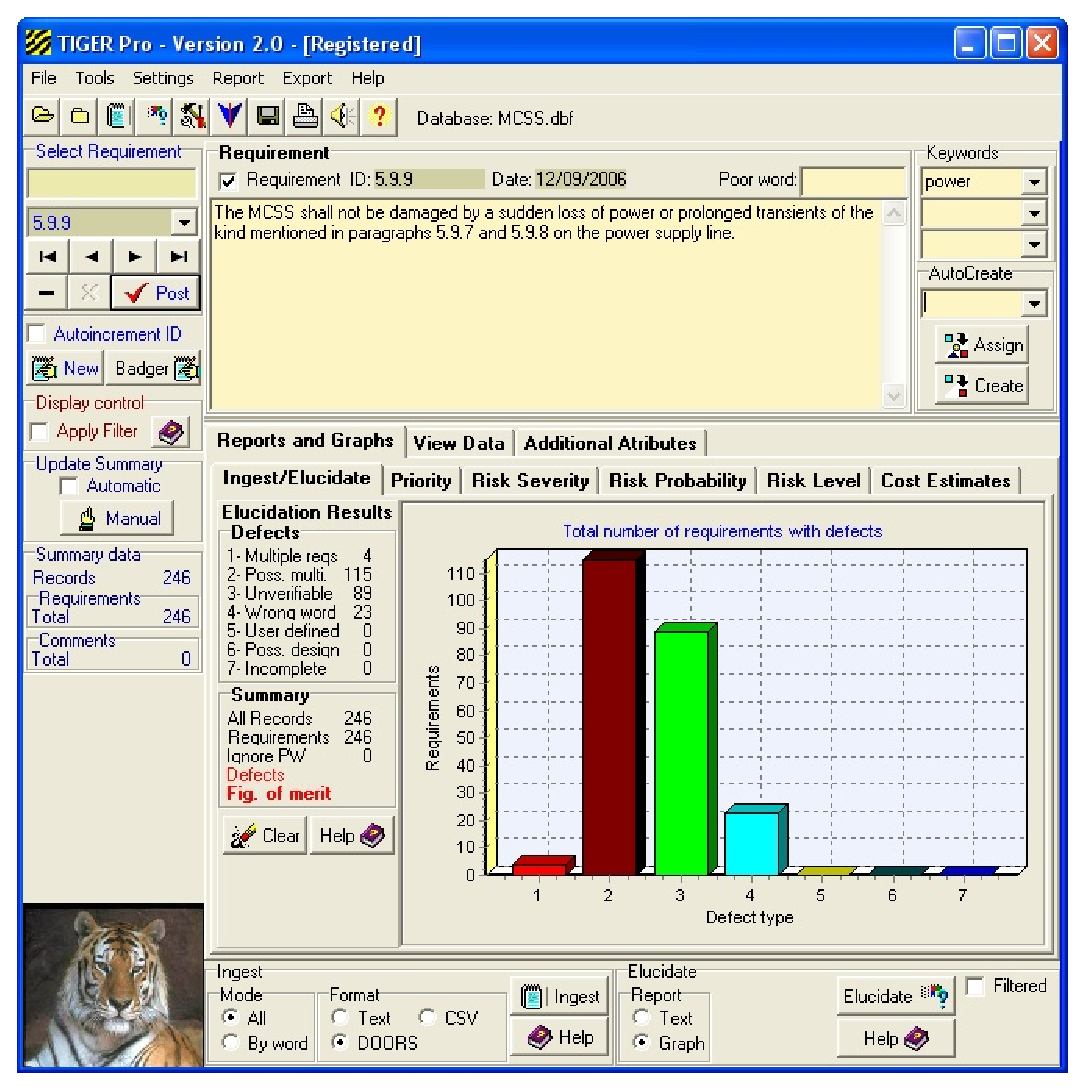
\includegraphics[scale=0.4]{figuras/ferramentas/tigerpro}
\caption{Visão exemplo da ferramenta TigerPRO}
\end{figure}
\newpage
\section{Resultados}

\begin{table}[!htpb]
\centering
\label{my-label}
\begin{tabular}{| l | c | c | l |}
Critérios / Ferramenta & \multicolumn{1}{l}{Target Process} & \multicolumn{1}{l}{VersionOne}                               & TigerPro              \\
1                      & X                                  & X                                                            &                       \\
2                      & X                                  & X                                                            & \multicolumn{1}{c}{X} \\
3                      & X                                  & X                                                            & \multicolumn{1}{c}{X} \\
4                      & X                                  & X                                                            &                       \\
5                      & X                                  & X                                                            & \multicolumn{1}{c}{X} \\
6                      & X                                  & X                                                            & \multicolumn{1}{c}{X} \\
7                      & X                                  & X                                                            &                       \\
8                      & FREE                               & \begin{tabular}[c]{@{}c@{}}PREMIUM\\  COM TRIAL\end{tabular} & FREE                 
\end{tabular}
\caption{Tabela de correspondência dos critérios adotados e ferramentas analisadas}
\end{table}

\subsection{Ferramenta escolhida}
	As ferramentas VersionOne e TargetProcess corresponderam a todos os critérios, mas o fator de decisão foi a acessibilidade da TargetProcess que permite um número máximo de versões free por usuário, mas como só esse projeto será gerido, ela acaba por ser FREE, enquanto o trial da VersionOne é por contagem de dias.